%%%%%%%%%%%% Attribution %%%%%%%%%%%%
% This template was created by 
% Chuck F. Rocca at WCSU and may be
% copied and used freely for 
% non-commercial purposes.
% 10-17-2021
%%%%%%%%%%%%%%%%%%%%%%%%%%%%%%%%%%%%%

%%%%%%% Start Document Header %%%%%%%
% In creating a new document
% copy and paste the header 
% as is.
%%%%%%%%%%%%%%%%%%%%%%%%%%%%%%%%%%%%%

\documentclass{article}

%%%% Header Information %%%%
    %%% Document Settings %%%%
    \usepackage[utf8]{inputenc}
    \usepackage[
        twoside,
        top=1in,
        bottom=0.75in,
        inner=0.5in,
        outer=0.5in
    ]{geometry}
    \pagestyle{myheadings}

%%%% Additional Commands to Load %%%%
    \usepackage{tcolorbox}
    \tcbuselibrary{skins}
    \usepackage{minted}
    \usepackage{color}
    \usepackage{tikz}
    \usetikzlibrary{calc}
    \usepackage{tabularx,colortbl}
    \usepackage{amsfonts,amsmath,amssymb}
    \usepackage{titling}
    \usepackage{mathrsfs}
    \usepackage{calc}
    \usepackage{xepersian}

%%%% Commands to Define Homework Boxes %%%%
%%%% Box Definition %%%%
    \newtcolorbox{prob}[1]{
    % Set box style
        sidebyside,
        sidebyside align=bottom,
    % Dimensions and layout
        width=\textwidth,
        toptitle=2.5pt,
        bottomtitle=2.5pt,
        righthand width=0\textwidth,
    % Coloring
        colbacktitle=gray!30,
        coltitle=black,
        colback=white,
        colframe=white,
    % Title formatting
        title={
            #1 \hfill نمره:\phantom{WWWW}
        },
        fonttitle=\large\bfseries
    }

%%%% Environment Definition %%%%
    \newenvironment{problem}[1]{
        \begin{prob}{#1}
    }
    {
        \tcblower
        \centering
        \vspace{\baselineskip}
        \end{prob}
    }



%%%% Document Information %%%%
    \title{\lr{HW2 Solutions}}
    \author{\lr{Written By Reza Shahriari}}
    \date{}

%%%%%%% End Document Header %%%%%%%


%%%% Begin Document %%%%
% note that the document starts with
% \begin{document} and ends with
% \end{document}
%%%%%%%%%%%%%%%%%%%%%%%%
\settextfont{BNAZANIN.TTF}

\begin{document}

%%%% Format Running Header %%%%%
\markboth{\theauthor}{\thetitle}

%%%% Insert the Title Information %%%
\maketitle


%%%% General Description of the Document %%%%


\raggedleft
%%%% Introduction to the General Template %%%%
\section{بخش مقدماتی (35 نمره)}
\centering
\lr{Disclaimer:} 

\lr{This is the solution manual to the homework assigned to students of Digital Control - Dr.Talebi.}

\lr{We do not guarantee that this solution is precise and thorough so please contact your TA to propose your innovative solutions and/or any probable mistakes.}


    \begin{problem}{سوال اول}
    \raggedleft
    \lr{Solution:}
    
    $\frac{X(z)}{z} = \frac{2z^2+1}{(z-2)^2(z-1)} = \frac{9}{(z-2)^2} - \frac{1}{z-2} + \frac{3}{z-1}$
    
    \lr{then}
    
    $X(z) = \frac{9z^{-1}}{(1-2z^-1)^2} - \frac{1}{1-2z^-1} + \frac{3}{1-z^-1}$
    
    \lr{At last we have} :
    
    $x(k) = 9k(2^{k-1}) - 2^k + 3$
    
    
    \end{problem}

    \begin{problem}{سوال دوم}
    \raggedleft
    \lr{Firstly : Decompose the Transfer function to the following :}
    
    $G(z)  = \frac{1}{z-0.1} \frac{z-2}{z^2 - 0.5z +1}$
    
    \lr{Realize the first part:}
    
    $G_{FP} = \frac{z^{-1}}{1-0.1z^{-1}}$
    
    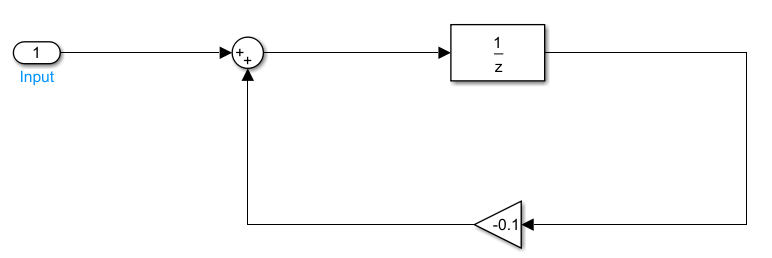
\includegraphics[width=\linewidth]{Second Series/8.png}
    
    \lr{Now Realize the second part:}
    
    $G_{ُSP} =\frac{z^{-1} - 2z^{-2}}{1 - 0.5z{-1} +z{-2}}$
    
    \lr{Use Observable Canonical :}
    
    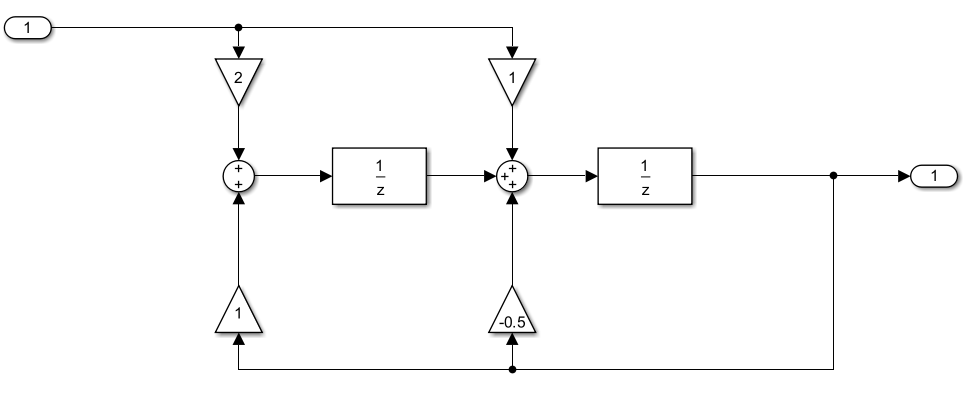
\includegraphics[width=\linewidth]{Second Series/9.png}
    
    \lr{Bring the two realized parts together to have the realized block diagram.}
    
    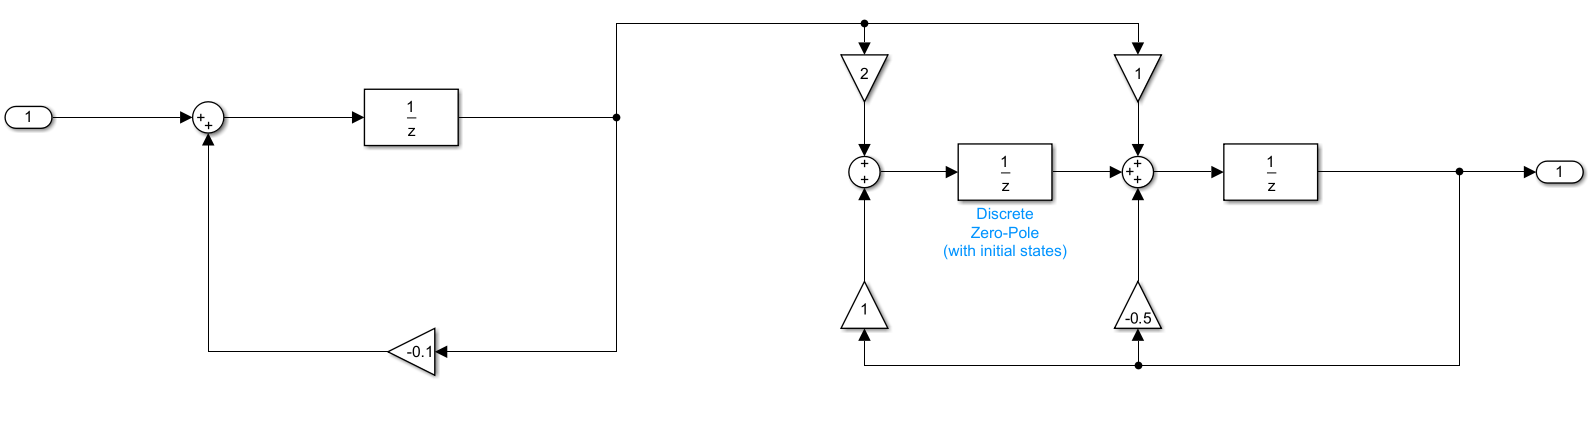
\includegraphics[width=\linewidth]{Second Series/10.png}
    	
    	
    	 
    \end{problem}
    
    \begin{problem}{سوال سوم}
    	\raggedleft
    	$-\frac{1}{s}U(s)e^{-sT} + \frac{1}{s}U(s) = Y(s)$
    	
    	\lr{The transfer function would be:}
    	
    	$G(s) = \frac{1-e^{-sT}}{s}$ 
    	
    	\lr{This is the ZOH transfer function.}
    	
    \end{problem}
    \begin{figure}[htbp]
    	\centering
    	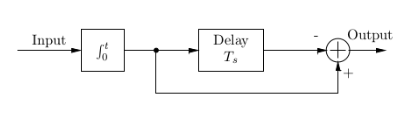
\includegraphics{Second Series/4.png}
    	\caption{شکل سوال سوم}
    \end{figure}
    
    
    \begin{problem}{سوال چهارم}
    	
    	
    \end{problem}
    \begin{figure}[htbp]
    	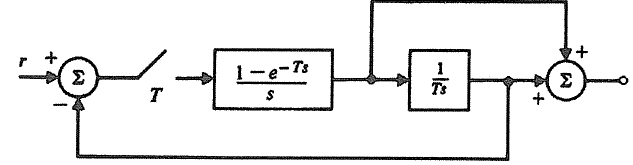
\includegraphics[width=\linewidth]{Second Series/5.png}
    	\caption{شکل سوال چهارم}
    \end{figure}
    
    \begin{problem}{سوال پنجم}
    	
    	
    \end{problem}
\raggedleft    
\section{بخش متوسط (35 نمره)}
\centering
حل \underline{دو سوال} از این بخش الزامی است.
\begin{problem}{سوال ششم}
	

\end{problem}
	

\begin{problem}{سوال هفتم}
	
	
	
\end{problem}
\begin{figure}
	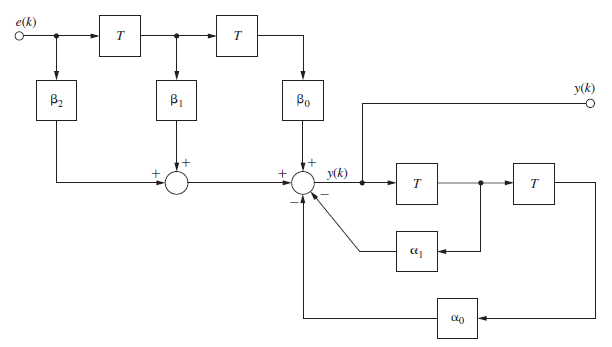
\includegraphics[width=\linewidth]{Second Series/2.png}
	\caption{شکل سوال هفتم}
\end{figure}

\begin{problem}{سوال هشتم}




\end{problem}
\begin{figure}
	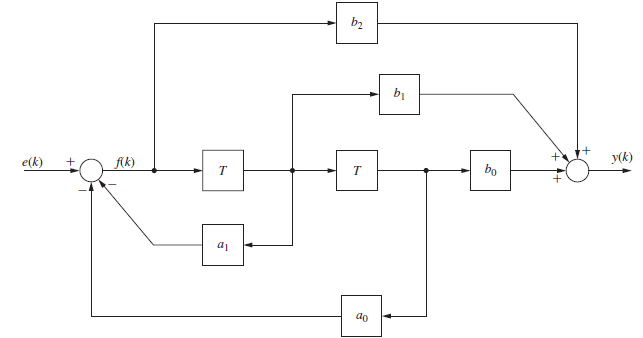
\includegraphics[width=\linewidth]{Second Series/3.png}
	\caption{شکل سوال هشتم}
\end{figure}


\begin{problem}{سوال نهم}





\end{problem}


\begin{problem}{سوال دهم}
	
	
	
	
\end{problem}


\raggedleft
\section{ بخش تکمیلی (30 نمره)}
\centering
حل \underline{دو سوال} از این بخش الزامی است.
\begin{problem}{سوال یازدهم}
	
	
	
\end{problem}
\begin{figure}[htbp]
	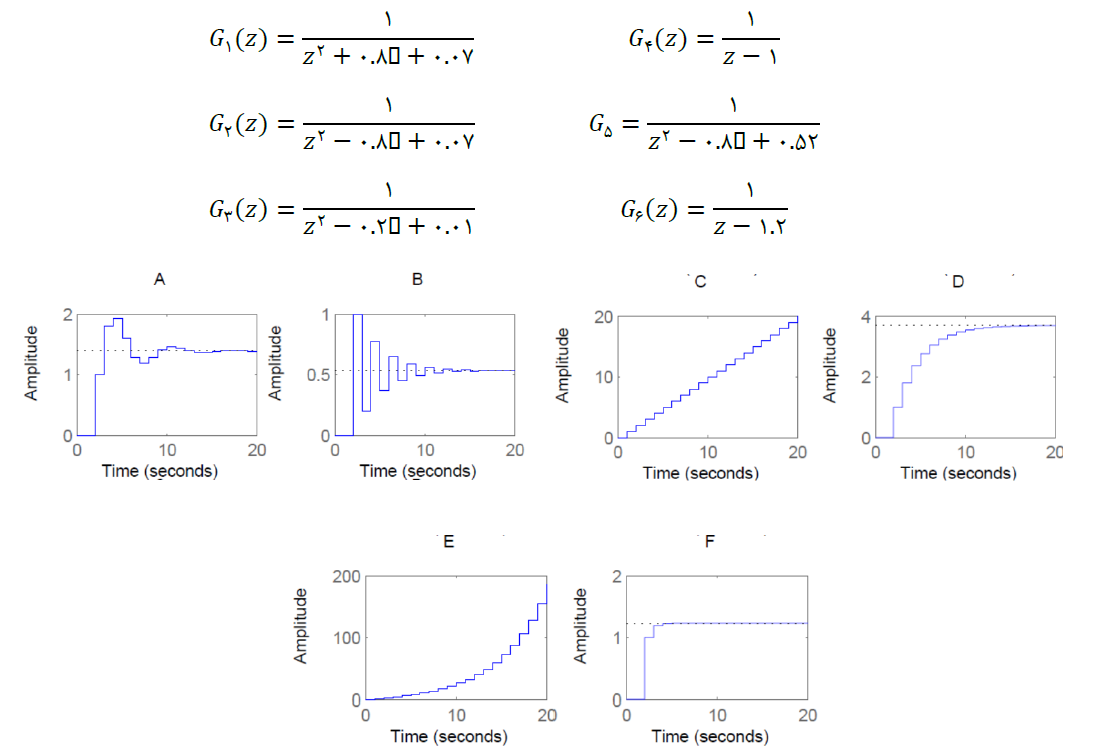
\includegraphics[width=\linewidth]{Second Series/1.png}
	\caption{شکل سوال یازدهم}
\end{figure}


\begin{problem}{سوال دوازدهم}



\end{problem}
\begin{figure}
	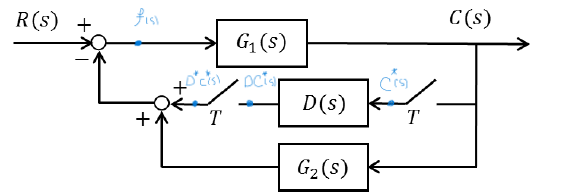
\includegraphics[width=\linewidth]{Second Series/6.png}
	\caption{شکل سوال دوازدهم}
\end{figure}


\begin{problem}{سوال سیزدهم}
	
	
	
	
	
\end{problem}
\begin{figure}
	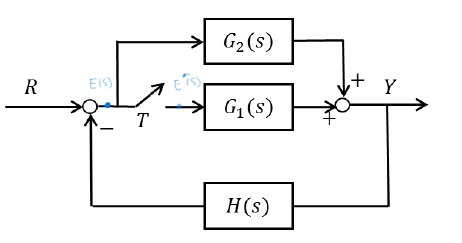
\includegraphics[width=\linewidth]{Second Series/7.png}
	\caption{شکل سوال سیزدهم}
\end{figure}

\begin{problem}{سوال چهاردهم}
	
	
	
	
	
\end{problem}


\begin{problem}{سوال پانزدهم}
	
	
	
	
	
\end{problem}


\end{document}
